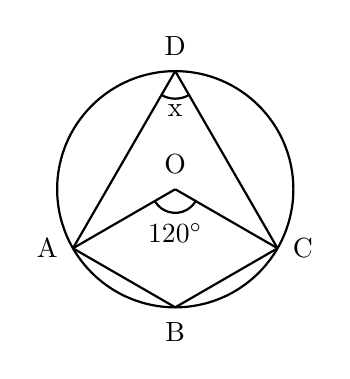
\begin{tikzpicture}[scale=1]

    % Define the center of the circle
    \coordinate (O) at (0,0);

    % Draw the circle
    \draw[thick] (O) circle (1.5);

    % Define points on the circle
    \coordinate (A) at (210:1.5);
    \coordinate (B) at (270:1.5);
    \coordinate (C) at (330:1.5);
    \coordinate (D) at (90:1.5);

    % Draw the lines and segments
    \draw[thick] (A) -- (D);
    \draw[thick] (A) -- (B);
    \draw[thick] (D) -- (C);
    \draw[thick] (B) -- (C);
    \draw[thick] (O) -- (A);
    \draw[thick] (O) -- (C);

    % Draw the angle arcs
    % Arc at O (between OA at 210 degrees and OC at 330 degrees)
    \draw[thick] (O) ++(210:0.3) arc (210:330:0.3);
    
    % Arc at D (between DA at 240 degrees and DC at 300 degrees)
    \draw[thick] (D) ++(240:0.35) arc (240:300:0.35);

    % Add labels for the points
    \node[left, xshift=-2pt] at (A) {A};
    \node[below, yshift=-2pt] at (B) {B};
    \node[right, xshift=2pt] at (C) {C};
    % Positioned O slightly above its coordinate to avoid the angle arc
    \node[above, yshift=2pt] at (O) {O}; 
    \node[above, yshift=2pt] at (D) {D};

    % Add angle values
    \node at (270:0.55) {$120^{\circ}$};
    \node at (90:1.0) {x};

\end{tikzpicture}